\documentclass[11pt]{article}
\usepackage[margin=1in]{geometry}
\usepackage{booktabs}
\usepackage{graphicx}
\usepackage{amsmath,amssymb}
\usepackage{xcolor}
\usepackage[hidelinks]{hyperref}
\usepackage{caption}
\usepackage{subcaption}
\usepackage{enumitem}
\usepackage{tabularx}
\usepackage{float}
\usepackage{pifont}
\usepackage{tikz}
\usetikzlibrary{arrows.meta, shadings}
\definecolor{feltdark}{HTML}{1B4D30}

\newcommand{\bx}[1]{#1$\times$#1}
% "Appendix A" as one link (not just the letter)
\newcommand{\appref}[1]{\hyperref[#1]{Appendix~\ref*{#1}}}
\newcommand{\pending}[1]{\noindent\fcolorbox{gray}{gray!8}{\parbox{\dimexpr\linewidth-2\fboxsep-2\fboxrule}{\small\textbf{Status: training in progress.} #1}}}
\newcommand{\flag}[1]{\noindent\fcolorbox{red!60!black}{red!5}{\parbox{\dimexpr\linewidth-2\fboxsep-2\fboxrule}{\small #1}}}

\newcommand{\NumCandidates}{96}

\newcommand{\RuleMultiMove}{b3}
\newcommand{\RuleMultiDirs}{3}
\newcommand{\RuleMultiFlips}{3}
\newcommand{\RulePassMover}{Black}
\newcommand{\RulePassOther}{White}
\newcommand{\RuleEndBlack}{20}
\newcommand{\RuleEndWhite}{16}

\newcommand{\StartValue}{-0.63}
\newcommand{\OrolettoRun}{seed1}

\newcommand{\NumTests}{48}

\newcommand{\TrainGames}{200{,}000}

\makeatletter
\newcommand{\tabinput}[1]{\@@input #1 }
\makeatother

% ---- Othello board diagrams -------------------------------------------
% \othboard{black discs}{white discs}{legal-move marks}{ringed squares}
% Each list is col/row pairs (1-based, col 1 = a, row 1 = top); use {} for none.
\definecolor{felt}{HTML}{2E7D4F}
\newcommand{\othboard}[4]{%
\begin{tikzpicture}[scale=0.5]
  \fill[felt] (0,0) rectangle (6,-6);
  \foreach \i in {0,...,6} {\draw[black!60] (\i,0) -- (\i,-6); \draw[black!60] (0,-\i) -- (6,-\i);}
  \foreach \l [count=\i] in {a,b,c,d,e,f} \node[font=\scriptsize] at (\i-0.5,0.45) {\l};
  \foreach \i in {1,...,6} \node[font=\scriptsize] at (-0.45,-\i+0.5) {\i};
  \def\lst{#1}\ifx\lst\empty\else\foreach \c/\r in {#1} \fill[black] (\c-0.5,-\r+0.5) circle (0.38);\fi
  \def\lst{#2}\ifx\lst\empty\else\foreach \c/\r in {#2} {\fill[white] (\c-0.5,-\r+0.5) circle (0.38); \draw[black!70] (\c-0.5,-\r+0.5) circle (0.38);}\fi
  \def\lst{#3}\ifx\lst\empty\else\foreach \c/\r in {#3} \fill[yellow!80!orange] (\c-0.5,-\r+0.5) circle (0.17);\fi
  \def\lst{#4}\ifx\lst\empty\else\foreach \c/\r in {#4} \draw[red!80!black, very thick] (\c-0.5,-\r+0.5) circle (0.46);\fi
\end{tikzpicture}}

\title{Learning to Learn Othello:\\Rule-Based Bots, Classical Reinforcement Learning and Beyond}
\author{Palak Raisinghani}
\date{\today}

\begin{document}
\tikzset{
  board/.style={fill=felt, draw=feltdark, line width=1.2pt},
  grid/.style={feltdark, line width=0.5pt},
  bdisc/.style={circle, inner sep=0pt, minimum size=7.4mm, ball color=black!85, draw=black},
  wdisc/.style={circle, inner sep=0pt, minimum size=7.4mm, ball color=white, draw=black!55},
  shadow/.style={circle, inner sep=0pt, minimum size=7.4mm, fill=black!45, opacity=0.35},
  ghostb/.style={circle, inner sep=0pt, minimum size=6mm, draw=black, dashed, line width=0.9pt},
  ghostw/.style={circle, inner sep=0pt, minimum size=6mm, draw=white, dashed, line width=0.9pt},
  newmark/.style={circle, inner sep=0pt, minimum size=8.6mm, draw=red!75!black, line width=1.6pt},
  flipmark/.style={circle, inner sep=0pt, minimum size=8.6mm, draw=orange!95!black, line width=1.4pt},
  capture/.style={-{Stealth[length=2.2mm]}, red!75!black, line width=1.6pt, opacity=0.85, shorten >=1.5mm, shorten <=3.2mm},
  illegal/.style={red!75!black, line width=2pt},
  coord/.style={font=\large\sffamily, text=black!75},
  halo/.style={white, line width=3.4pt, opacity=0.75, shorten >=1.5mm, shorten <=3.2mm},
}

\maketitle

\begin{abstract}
Othello has simple rules, but its strategy is deep and often counter-intuitive. Moves that bring high immediate rewards can prove to be harmful later, and moves that seem to be of no great immediate value can prove extremely beneficial later on in the game. Othello is thus a strong benchmark to prove capabilty in learning delayed rewards.
This project tests several different Rule Based and RL models on their ability to learn how to play Othello. Finally we develop a solid model for the game and offer an attractive interface to play the game against our RL-build Model that we call \textit{Oroletto}.

\end{abstract}

\tableofcontents

%======================================================================

\section{Why Reinforcement Learning for Games}
\label{sec:whyrl}

\subsection{Games as reinforcement-learning problems}
\hspace{2em} Reinforcement learning studies agents that learn to act by trial and error, in
order to maximise a cumulative reward \cite{sutton2018}. They learn better policies while interacting with the environment. To do so they balance exploration and exploitation. This project looks at the classic board game of Othello and trains a RL model for the same. Historically, programmers developed rule-based bots which operated on handwritten rules.\\
For complicated games, like chess, this was hard and a tree search based approach was adopted. These bots were capable of choosing optimal actions at each step but were very computationally expensive. \\
With the advent of RL, games and especially board games found a new player. Board games offer two
things that real-world RL problems rarely do:
\begin{itemize}[leftmargin=*]
  \item \textbf{A perfect, free simulator.} Rules are exact and games can be
        replayed millions of times, so data is limited only by compute.
  \item \textbf{Self-play.} An agent can play against copies of itself. It then
        always faces an opponent of its own strength, which produces an
        automatic curriculum without human data.
\end{itemize}
Games are also hard in a way that makes them useful benchmarks. The reward is
\emph{sparse} and \emph{delayed}: a single number after dozens of moves. The
learner must therefore solve the \emph{credit-assignment problem}, which is
working out which earlier moves caused the result. State spaces are also far too
large to tabulate, so the agent has to \emph{generalise} from positions it has
seen to positions it has not.

\subsection{Landmark game-playing systems}

\begin{table}[H]
\centering
\caption{Landmark game-playing systems. Not all of them use RL; Deep Blue is
included as the classic \emph{search-only} contrast.}
\label{tab:landmarks}
\small
\begin{tabularx}{\linewidth}{@{}llrX@{}}
\toprule
Game & System & Year & Core idea \\
\midrule
Checkers & Samuel's player \cite{samuel1959} & 1959 & Learned a linear evaluation by comparing it with deeper search; an early ancestor of temporal-difference learning. \\
Othello & IAGO \cite{rosenbloom1982} & 1982 & Hand-built evaluation that introduced mobility as a central concept. \\
Backgammon & TD-Gammon \cite{tesauro1995} & 1995 & A neural network trained by TD($\lambda$) through self-play; reached top human level. \\
Othello & Logistello \cite{buro1995,buro1997} & 1997 & Evaluation fitted by regression on pattern features from self-play games; beat the world champion 6--0. \\
Chess & Deep Blue \cite{campbell2002} & 1997 & Massive alpha-beta search with a hand-tuned evaluation; no learning. Beat Kasparov. \\
Atari & DQN \cite{mnih2015} & 2015 & Deep Q-learning from pixels, using experience replay and a target network. \\
Go & AlphaGo \cite{silver2016} & 2016 & Policy and value networks (supervised, then RL) guiding Monte Carlo tree search. \\
Go & AlphaGo Zero \cite{silver2017} & 2017 & Pure self-play from random play, with a single residual network plus MCTS. \\
Chess, shogi, Go & AlphaZero \cite{silver2018} & 2018 & The same algorithm and settings master all three games. \\
Dota 2 & OpenAI Five \cite{berner2019} & 2019 & Large-scale PPO self-play in a team game with hidden information. \\
StarCraft II & AlphaStar \cite{vinyals2019} & 2019 & Multi-agent RL with a league of past and exploiter agents. \\
Atari, board games & MuZero \cite{schrittwieser2020} & 2020 & AlphaZero-style planning with a \emph{learned} model of the rules. \\
Othello & Othello-GPT \cite{li2023} & 2023 & A sequence model trained on move lists forms an internal board representation. \\
\bottomrule
\end{tabularx}
\end{table}

Table~\ref{tab:landmarks} shows a clear trajectory. Early systems learned only
the \emph{weights} of hand-designed features (Samuel, Logistello). TD-Gammon
showed that a neural network could learn its own features from self-play. The
AlphaGo line then combined learned networks with \emph{search}: the network
supplies intuition about which moves are promising and how good a position is,
and tree search corrects the network's mistakes by looking ahead. Deep Blue is a
reminder that search alone, with expert-tuned evaluation, is already very strong.
This is why our ladder of rule-based bots (\S\ref{sec:bots}) includes a search
bot.

\subsection{Why Othello}
Othello sits at a useful point between toy problems and grand challenges. The
rules fit in three lines, but the state space is far beyond a lookup table even
on \bx{6}. Its strategy is also counter-intuitive: the disc-count trap
(\S\ref{sec:concepts}) means the obvious objective is the wrong one. This tests
whether a learner discovers the real structure of the game or only the surface
statistic. Finally, its small boards are solved, which gives ground truth that
large games like Go do not have.

%======================================================================

\section{Othello : The Board Game}
\label{sec:game}

\subsection{Board and pieces}
Othello is a two-player, zero-sum, perfect-information game played on an
$n\times n$ board, classically \bx{8} \cite{cs121}. The two opponents are
assigned colours, black and white, and play with discs that are black on one
side and white on the other. The game begins with two discs of each colour on
the four centre squares, placed diagonally (Fig.~\ref{fig:rules}a). The players
then alternate moves, with Black moving first.\footnote{The handout
\cite{cs121} lets White move first. The modern tournament convention, which this
project and its code follow, is that Black moves first. The two differ only in
which colour is called which.} We name squares by column letter and row
number, so on \bx{6} the corners are a1, f1, a6 and f6. The rules do not depend
on the board size, and this project uses \bx{6}, \bx{8} and \bx{10}.

\subsection{Rules}
The rules below follow the formulation of \cite{cs121}.
\begin{enumerate}[leftmargin=*]
  \item \textbf{Legal moves.} A move places one additional disc of your colour
        on an empty square. It is legal only if the new disc \emph{surrounds}
        one or more of the opponent's discs along a straight line, so that they
        lie between the new disc and another disc of your colour with no empty
        square in between. The line may run horizontally, vertically or
        diagonally. In other words, a move is legal only if at least one
        opponent disc is captured by it. On the very first move there are
        exactly four legal moves (Fig.~\ref{fig:rules}a).
  \item \textbf{Flipping.} Every surrounded opponent disc is replaced by a disc
        of your colour (in practice the disc is flipped over). This applies
        along \emph{every} line the new disc closes at once, not just one. In
        Fig.~\ref{fig:rules}b, Black plays c2, which surrounds the white disc
        on c3 against Black's disc on c4, so c3 becomes black;
        Fig.~\ref{fig:rules}c--d shows one move capturing along \RuleMultiDirs{}
        lines at once.
  \item \textbf{Forfeiting a turn.} A player must move whenever they have a
        legal move; a turn can never be forfeited voluntarily. If a player has
        \emph{no} legal move, their turn is forfeited (a \emph{pass}) and the
        opponent moves again (Fig.~\ref{fig:rules}e). A player may have to pass on several consecutive
        turns while the opponent keeps moving.
  \item \textbf{End of the game.} The game ends when every square is filled,
        or when neither player can make a legal move.
  \item \textbf{Winner.} When the game ends, the board is scored: the player
        with more discs of their colour wins (Fig.~\ref{fig:rules}f). Equal counts are a draw.
\end{enumerate}

\begin{figure}[H]
\centering
\begin{subfigure}[t]{0.48\linewidth}\centering
  \begin{tikzpicture}[scale=0.62, every node/.style={transform shape}]
\fill[board] (0,0) rectangle (6,6);
\draw[grid] (1,0) -- (1,6); \draw[grid] (0,1) -- (6,1);
\draw[grid] (2,0) -- (2,6); \draw[grid] (0,2) -- (6,2);
\draw[grid] (3,0) -- (3,6); \draw[grid] (0,3) -- (6,3);
\draw[grid] (4,0) -- (4,6); \draw[grid] (0,4) -- (6,4);
\draw[grid] (5,0) -- (5,6); \draw[grid] (0,5) -- (6,5);
\draw[feltdark, line width=1.2pt] (0,0) rectangle (6,6);
\node[coord] at (0.5,6.4) {a};
\node[coord] at (1.5,6.4) {b};
\node[coord] at (2.5,6.4) {c};
\node[coord] at (3.5,6.4) {d};
\node[coord] at (4.5,6.4) {e};
\node[coord] at (5.5,6.4) {f};
\node[coord] at (-0.4,5.5) {1};
\node[coord] at (-0.4,4.5) {2};
\node[coord] at (-0.4,3.5) {3};
\node[coord] at (-0.4,2.5) {4};
\node[coord] at (-0.4,1.5) {5};
\node[coord] at (-0.4,0.5) {6};
\node[shadow] at (2.56,3.43) {};
\node[wdisc] at (2.5,3.5) {};
\node[shadow] at (3.56,3.43) {};
\node[bdisc] at (3.5,3.5) {};
\node[shadow] at (2.56,2.43) {};
\node[bdisc] at (2.5,2.5) {};
\node[shadow] at (3.56,2.43) {};
\node[wdisc] at (3.5,2.5) {};
\node[ghostb] at (2.5,4.5) {};
\node[ghostb] at (1.5,3.5) {};
\node[ghostb] at (4.5,2.5) {};
\node[ghostb] at (3.5,1.5) {};
\draw[illegal] (4.22,1.22) -- (4.78,1.78) (4.22,1.78) -- (4.78,1.22);
\end{tikzpicture}

  \caption{\textbf{Start.} Two discs each, placed diagonally. Dashed
  circles: Black's four legal moves. \textcolor{red!75!black}{\ding{55}}~e5
  touches a white disc but surrounds nothing, so it is illegal.}
\end{subfigure}\hfill
\begin{subfigure}[t]{0.48\linewidth}\centering
  \begin{tikzpicture}[scale=0.62, every node/.style={transform shape}]
\fill[board] (0,0) rectangle (6,6);
\draw[grid] (1,0) -- (1,6); \draw[grid] (0,1) -- (6,1);
\draw[grid] (2,0) -- (2,6); \draw[grid] (0,2) -- (6,2);
\draw[grid] (3,0) -- (3,6); \draw[grid] (0,3) -- (6,3);
\draw[grid] (4,0) -- (4,6); \draw[grid] (0,4) -- (6,4);
\draw[grid] (5,0) -- (5,6); \draw[grid] (0,5) -- (6,5);
\draw[feltdark, line width=1.2pt] (0,0) rectangle (6,6);
\node[coord] at (0.5,6.4) {a};
\node[coord] at (1.5,6.4) {b};
\node[coord] at (2.5,6.4) {c};
\node[coord] at (3.5,6.4) {d};
\node[coord] at (4.5,6.4) {e};
\node[coord] at (5.5,6.4) {f};
\node[coord] at (-0.4,5.5) {1};
\node[coord] at (-0.4,4.5) {2};
\node[coord] at (-0.4,3.5) {3};
\node[coord] at (-0.4,2.5) {4};
\node[coord] at (-0.4,1.5) {5};
\node[coord] at (-0.4,0.5) {6};
\node[shadow] at (2.56,4.43) {};
\node[bdisc] at (2.5,4.5) {};
\node[shadow] at (2.56,3.43) {};
\node[bdisc] at (2.5,3.5) {};
\node[shadow] at (3.56,3.43) {};
\node[bdisc] at (3.5,3.5) {};
\node[shadow] at (2.56,2.43) {};
\node[bdisc] at (2.5,2.5) {};
\node[shadow] at (3.56,2.43) {};
\node[wdisc] at (3.5,2.5) {};
\node[flipmark] at (2.5,3.5) {};
\node[newmark] at (2.5,4.5) {};
\draw[halo] (2.5,4.5) -- (2.5,2.5);
\draw[capture] (2.5,4.5) -- (2.5,2.5);
\end{tikzpicture}

  \caption{\textbf{A capture.} Black plays c2 (red ring). The white disc on
  c3 lies between c2 and Black's c4 (arrow), so it flips (orange ring).}
\end{subfigure}

\vspace{4mm}
\begin{subfigure}[t]{0.48\linewidth}\centering
  \begin{tikzpicture}[scale=0.62, every node/.style={transform shape}]
\fill[board] (0,0) rectangle (6,6);
\draw[grid] (1,0) -- (1,6); \draw[grid] (0,1) -- (6,1);
\draw[grid] (2,0) -- (2,6); \draw[grid] (0,2) -- (6,2);
\draw[grid] (3,0) -- (3,6); \draw[grid] (0,3) -- (6,3);
\draw[grid] (4,0) -- (4,6); \draw[grid] (0,4) -- (6,4);
\draw[grid] (5,0) -- (5,6); \draw[grid] (0,5) -- (6,5);
\draw[feltdark, line width=1.2pt] (0,0) rectangle (6,6);
\node[coord] at (0.5,6.4) {a};
\node[coord] at (1.5,6.4) {b};
\node[coord] at (2.5,6.4) {c};
\node[coord] at (3.5,6.4) {d};
\node[coord] at (4.5,6.4) {e};
\node[coord] at (5.5,6.4) {f};
\node[coord] at (-0.4,5.5) {1};
\node[coord] at (-0.4,4.5) {2};
\node[coord] at (-0.4,3.5) {3};
\node[coord] at (-0.4,2.5) {4};
\node[coord] at (-0.4,1.5) {5};
\node[coord] at (-0.4,0.5) {6};
\node[shadow] at (3.56,5.43) {};
\node[bdisc] at (3.5,5.5) {};
\node[shadow] at (1.56,4.43) {};
\node[wdisc] at (1.5,4.5) {};
\node[shadow] at (2.56,4.43) {};
\node[wdisc] at (2.5,4.5) {};
\node[shadow] at (3.56,4.43) {};
\node[bdisc] at (3.5,4.5) {};
\node[shadow] at (2.56,3.43) {};
\node[wdisc] at (2.5,3.5) {};
\node[shadow] at (3.56,3.43) {};
\node[bdisc] at (3.5,3.5) {};
\node[shadow] at (2.56,2.43) {};
\node[wdisc] at (2.5,2.5) {};
\node[shadow] at (3.56,2.43) {};
\node[bdisc] at (3.5,2.5) {};
\node[shadow] at (2.56,1.43) {};
\node[wdisc] at (2.5,1.5) {};
\node[shadow] at (3.56,1.43) {};
\node[bdisc] at (3.5,1.5) {};
\node[shadow] at (4.56,1.43) {};
\node[bdisc] at (4.5,1.5) {};
\node[shadow] at (4.56,0.43) {};
\node[bdisc] at (4.5,0.5) {};
\node[ghostb] at (1.5,3.5) {};
\draw[halo] (1.5,3.5) -- (3.5,5.5);
\draw[capture] (1.5,3.5) -- (3.5,5.5);
\draw[halo] (1.5,3.5) -- (3.5,3.5);
\draw[capture] (1.5,3.5) -- (3.5,3.5);
\draw[halo] (1.5,3.5) -- (3.5,1.5);
\draw[capture] (1.5,3.5) -- (3.5,1.5);
\end{tikzpicture}

  \caption{\textbf{Several lines at once (before).} Black to move. Playing
  \RuleMultiMove{} (dashed) closes \RuleMultiDirs{} lines at once; each arrow
  runs from the new disc to the black disc that anchors the line.}
\end{subfigure}\hfill
\begin{subfigure}[t]{0.48\linewidth}\centering
  \begin{tikzpicture}[scale=0.62, every node/.style={transform shape}]
\fill[board] (0,0) rectangle (6,6);
\draw[grid] (1,0) -- (1,6); \draw[grid] (0,1) -- (6,1);
\draw[grid] (2,0) -- (2,6); \draw[grid] (0,2) -- (6,2);
\draw[grid] (3,0) -- (3,6); \draw[grid] (0,3) -- (6,3);
\draw[grid] (4,0) -- (4,6); \draw[grid] (0,4) -- (6,4);
\draw[grid] (5,0) -- (5,6); \draw[grid] (0,5) -- (6,5);
\draw[feltdark, line width=1.2pt] (0,0) rectangle (6,6);
\node[coord] at (0.5,6.4) {a};
\node[coord] at (1.5,6.4) {b};
\node[coord] at (2.5,6.4) {c};
\node[coord] at (3.5,6.4) {d};
\node[coord] at (4.5,6.4) {e};
\node[coord] at (5.5,6.4) {f};
\node[coord] at (-0.4,5.5) {1};
\node[coord] at (-0.4,4.5) {2};
\node[coord] at (-0.4,3.5) {3};
\node[coord] at (-0.4,2.5) {4};
\node[coord] at (-0.4,1.5) {5};
\node[coord] at (-0.4,0.5) {6};
\node[shadow] at (3.56,5.43) {};
\node[bdisc] at (3.5,5.5) {};
\node[shadow] at (1.56,4.43) {};
\node[wdisc] at (1.5,4.5) {};
\node[shadow] at (2.56,4.43) {};
\node[bdisc] at (2.5,4.5) {};
\node[shadow] at (3.56,4.43) {};
\node[bdisc] at (3.5,4.5) {};
\node[shadow] at (1.56,3.43) {};
\node[bdisc] at (1.5,3.5) {};
\node[shadow] at (2.56,3.43) {};
\node[bdisc] at (2.5,3.5) {};
\node[shadow] at (3.56,3.43) {};
\node[bdisc] at (3.5,3.5) {};
\node[shadow] at (2.56,2.43) {};
\node[bdisc] at (2.5,2.5) {};
\node[shadow] at (3.56,2.43) {};
\node[bdisc] at (3.5,2.5) {};
\node[shadow] at (2.56,1.43) {};
\node[wdisc] at (2.5,1.5) {};
\node[shadow] at (3.56,1.43) {};
\node[bdisc] at (3.5,1.5) {};
\node[shadow] at (4.56,1.43) {};
\node[bdisc] at (4.5,1.5) {};
\node[shadow] at (4.56,0.43) {};
\node[bdisc] at (4.5,0.5) {};
\node[flipmark] at (2.5,4.5) {};
\node[flipmark] at (2.5,3.5) {};
\node[flipmark] at (2.5,2.5) {};
\node[newmark] at (1.5,3.5) {};
\end{tikzpicture}

  \caption{\textbf{Several lines at once (after).} All \RuleMultiFlips{}
  surrounded discs flip together, one per line.}
\end{subfigure}

\vspace{4mm}
\begin{subfigure}[t]{0.48\linewidth}\centering
  \begin{tikzpicture}[scale=0.62, every node/.style={transform shape}]
\fill[board] (0,0) rectangle (6,6);
\draw[grid] (1,0) -- (1,6); \draw[grid] (0,1) -- (6,1);
\draw[grid] (2,0) -- (2,6); \draw[grid] (0,2) -- (6,2);
\draw[grid] (3,0) -- (3,6); \draw[grid] (0,3) -- (6,3);
\draw[grid] (4,0) -- (4,6); \draw[grid] (0,4) -- (6,4);
\draw[grid] (5,0) -- (5,6); \draw[grid] (0,5) -- (6,5);
\draw[feltdark, line width=1.2pt] (0,0) rectangle (6,6);
\node[coord] at (0.5,6.4) {a};
\node[coord] at (1.5,6.4) {b};
\node[coord] at (2.5,6.4) {c};
\node[coord] at (3.5,6.4) {d};
\node[coord] at (4.5,6.4) {e};
\node[coord] at (5.5,6.4) {f};
\node[coord] at (-0.4,5.5) {1};
\node[coord] at (-0.4,4.5) {2};
\node[coord] at (-0.4,3.5) {3};
\node[coord] at (-0.4,2.5) {4};
\node[coord] at (-0.4,1.5) {5};
\node[coord] at (-0.4,0.5) {6};
\node[shadow] at (0.56,5.43) {};
\node[wdisc] at (0.5,5.5) {};
\node[shadow] at (1.56,5.43) {};
\node[wdisc] at (1.5,5.5) {};
\node[shadow] at (2.56,5.43) {};
\node[wdisc] at (2.5,5.5) {};
\node[shadow] at (1.56,4.43) {};
\node[bdisc] at (1.5,4.5) {};
\node[shadow] at (0.56,3.43) {};
\node[wdisc] at (0.5,3.5) {};
\node[shadow] at (1.56,3.43) {};
\node[bdisc] at (1.5,3.5) {};
\node[shadow] at (2.56,3.43) {};
\node[bdisc] at (2.5,3.5) {};
\node[shadow] at (3.56,3.43) {};
\node[bdisc] at (3.5,3.5) {};
\node[shadow] at (1.56,2.43) {};
\node[bdisc] at (1.5,2.5) {};
\node[shadow] at (2.56,2.43) {};
\node[bdisc] at (2.5,2.5) {};
\node[shadow] at (3.56,2.43) {};
\node[bdisc] at (3.5,2.5) {};
\node[shadow] at (4.56,1.43) {};
\node[bdisc] at (4.5,1.5) {};
\node[ghostw] at (4.5,3.5) {};
\node[ghostw] at (1.5,1.5) {};
\node[ghostw] at (2.5,1.5) {};
\node[ghostw] at (5.5,0.5) {};
\end{tikzpicture}

  \caption{\textbf{A forced pass.} It is \RulePassMover's turn, but no empty
  square surrounds a \RulePassOther{} disc, so \RulePassMover{} must pass and
  \RulePassOther{} moves again (dashed: \RulePassOther's legal moves).}
\end{subfigure}\hfill
\begin{subfigure}[t]{0.48\linewidth}\centering
  \begin{tikzpicture}[scale=0.62, every node/.style={transform shape}]
\fill[board] (0,0) rectangle (6,6);
\draw[grid] (1,0) -- (1,6); \draw[grid] (0,1) -- (6,1);
\draw[grid] (2,0) -- (2,6); \draw[grid] (0,2) -- (6,2);
\draw[grid] (3,0) -- (3,6); \draw[grid] (0,3) -- (6,3);
\draw[grid] (4,0) -- (4,6); \draw[grid] (0,4) -- (6,4);
\draw[grid] (5,0) -- (5,6); \draw[grid] (0,5) -- (6,5);
\draw[feltdark, line width=1.2pt] (0,0) rectangle (6,6);
\node[coord] at (0.5,6.4) {a};
\node[coord] at (1.5,6.4) {b};
\node[coord] at (2.5,6.4) {c};
\node[coord] at (3.5,6.4) {d};
\node[coord] at (4.5,6.4) {e};
\node[coord] at (5.5,6.4) {f};
\node[coord] at (-0.4,5.5) {1};
\node[coord] at (-0.4,4.5) {2};
\node[coord] at (-0.4,3.5) {3};
\node[coord] at (-0.4,2.5) {4};
\node[coord] at (-0.4,1.5) {5};
\node[coord] at (-0.4,0.5) {6};
\node[shadow] at (0.56,5.43) {};
\node[wdisc] at (0.5,5.5) {};
\node[shadow] at (1.56,5.43) {};
\node[wdisc] at (1.5,5.5) {};
\node[shadow] at (2.56,5.43) {};
\node[bdisc] at (2.5,5.5) {};
\node[shadow] at (3.56,5.43) {};
\node[bdisc] at (3.5,5.5) {};
\node[shadow] at (4.56,5.43) {};
\node[bdisc] at (4.5,5.5) {};
\node[shadow] at (5.56,5.43) {};
\node[wdisc] at (5.5,5.5) {};
\node[shadow] at (0.56,4.43) {};
\node[bdisc] at (0.5,4.5) {};
\node[shadow] at (1.56,4.43) {};
\node[wdisc] at (1.5,4.5) {};
\node[shadow] at (2.56,4.43) {};
\node[bdisc] at (2.5,4.5) {};
\node[shadow] at (3.56,4.43) {};
\node[bdisc] at (3.5,4.5) {};
\node[shadow] at (4.56,4.43) {};
\node[bdisc] at (4.5,4.5) {};
\node[shadow] at (5.56,4.43) {};
\node[wdisc] at (5.5,4.5) {};
\node[shadow] at (0.56,3.43) {};
\node[bdisc] at (0.5,3.5) {};
\node[shadow] at (1.56,3.43) {};
\node[bdisc] at (1.5,3.5) {};
\node[shadow] at (2.56,3.43) {};
\node[wdisc] at (2.5,3.5) {};
\node[shadow] at (3.56,3.43) {};
\node[bdisc] at (3.5,3.5) {};
\node[shadow] at (4.56,3.43) {};
\node[bdisc] at (4.5,3.5) {};
\node[shadow] at (5.56,3.43) {};
\node[wdisc] at (5.5,3.5) {};
\node[shadow] at (0.56,2.43) {};
\node[bdisc] at (0.5,2.5) {};
\node[shadow] at (1.56,2.43) {};
\node[bdisc] at (1.5,2.5) {};
\node[shadow] at (2.56,2.43) {};
\node[bdisc] at (2.5,2.5) {};
\node[shadow] at (3.56,2.43) {};
\node[wdisc] at (3.5,2.5) {};
\node[shadow] at (4.56,2.43) {};
\node[wdisc] at (4.5,2.5) {};
\node[shadow] at (5.56,2.43) {};
\node[bdisc] at (5.5,2.5) {};
\node[shadow] at (0.56,1.43) {};
\node[bdisc] at (0.5,1.5) {};
\node[shadow] at (1.56,1.43) {};
\node[bdisc] at (1.5,1.5) {};
\node[shadow] at (2.56,1.43) {};
\node[bdisc] at (2.5,1.5) {};
\node[shadow] at (3.56,1.43) {};
\node[wdisc] at (3.5,1.5) {};
\node[shadow] at (4.56,1.43) {};
\node[bdisc] at (4.5,1.5) {};
\node[shadow] at (5.56,1.43) {};
\node[wdisc] at (5.5,1.5) {};
\node[shadow] at (0.56,0.43) {};
\node[bdisc] at (0.5,0.5) {};
\node[shadow] at (1.56,0.43) {};
\node[wdisc] at (1.5,0.5) {};
\node[shadow] at (2.56,0.43) {};
\node[wdisc] at (2.5,0.5) {};
\node[shadow] at (3.56,0.43) {};
\node[wdisc] at (3.5,0.5) {};
\node[shadow] at (4.56,0.43) {};
\node[wdisc] at (4.5,0.5) {};
\node[shadow] at (5.56,0.43) {};
\node[wdisc] at (5.5,0.5) {};
\end{tikzpicture}

  \caption{\textbf{End of the game.} The board is full, so the game is over.
  Black has \RuleEndBlack{} discs and White \RuleEndWhite{}: Black wins.}
\end{subfigure}
\caption{The rules of Othello on a \bx{6} board. Every position comes from the
game engine (\texttt{scripts/make\_rule\_diagrams.py}), so each one is legal and
correctly flipped. Panels (a)--(b) are the same example as the interactive
tutorial (\texttt{othello --tutorial}, \S\ref{sec:cli}).}
\label{fig:rules}
\end{figure}

\subsection{Strategic concepts}
\label{sec:concepts}
Four ideas recur throughout this report. Each is defined here once. They also are the reason Othello is an attractive board game to experiment RL models on. 
\begin{description}[leftmargin=1.2em,style=nextline]
  \item[Stability and corners.] A disc is \emph{stable} if it can never be
  flipped again. A corner disc is always stable, because no line can sandwich
  it. A stable corner also lets the discs along its edges become stable.
  \item[X- and C-squares.] The squares diagonally adjacent (X) and orthogonally
  adjacent (C) to a corner. Playing there while the corner is empty tends to
  give the corner to the opponent.
  \item[Mobility.] The number of legal moves a player has. Keeping your own
  mobility high and the opponent's low eventually forces the opponent onto
  X- and C-squares.
  \item[The disc-count trap.] Owning many discs in the middle game is usually a
  \emph{weakness}. It flips discs the opponent can flip back, and it gives the
  opponent more moves. Only the final count matters, so maximising discs early
  is a classic beginner's error. This error turns out to matter for learning
  agents as well.
\end{description}

\subsection{Board size and solved results}
\bx{8} Othello has roughly $10^{28}$ legal positions and a game tree of about
$10^{58}$ \cite{allis1994}. It was only recently weakly solved, as a draw under
perfect play \cite{takizawa2023}. The \bx{6} game was solved much earlier: it is a
win for the second player (White), 16--20 \cite{feinstein1993}. We start on \bx{6}
because games are short and simulation is cheap. The board is still far too
large to enumerate, so it remains a real learning problem.

%======================================================================
\section{Rule-Based Bots}
\label{sec:bots}
Rule based bots are those that don't need any learning and have clear hand written rules. We use these as a benchmark for our RL models described later in the report. 3 rule based bots work on different general ideas and have been adapted to Othello for the purpose of this project.
Every learning method is judged against fixed, rule-based opponents.We compare the performance of these three bots and rate them according to the ELO rating. We also consider the three bots for three different board sizes and compare and rate them for the three different board sizes independently.
In this section we use the shared evaluation protocol summarised below and
detailed in \S\ref{sec:protocol}.
j
\paragraph{Evaluation protocol (summary).} Every match is played from $K$
openings of six random plies, and each opening is played once with each colour.
We report the \emph{score} (win $=1$, draw $=\tfrac12$) with a 95\% confidence
interval, the win rate and the mean final disc margin.

\subsection{The random bot}
The random bot plays a uniformly random legal move. It is the floor of the
ladder: any agent that has learned anything should beat it clearly. It also
calibrates the game itself. Under random play the first mover scores slightly
below half on every board size (Table~\ref{tab:throughput}), so evaluations
must alternate colours.

\subsection{The heuristic bot}
\label{sec:heuristic}
The heuristic bot is \emph{greedy}. For each legal move it evaluates the
resulting position with a hand-written evaluation function and plays the
best-scoring move. It looks exactly one ply ahead. The evaluation is a weighted
sum of four features, each computed as ``own minus opponent'' and defined for
any board size (Table~\ref{tab:heuristic_weights}):
\begin{itemize}[leftmargin=*]
  \item \textbf{Corners}: corner discs can never be flipped. They are
        \emph{stable} and anchor the stable discs along their edges.
  \item \textbf{Mobility}: the number of legal moves available. High mobility
        means many options. Low opponent mobility forces the opponent into
        bad squares.
  \item \textbf{Disc count}: material on the board.
  \item \textbf{X-squares}: discs diagonally adjacent to an \emph{empty}
        corner. Such a disc typically hands that corner to the opponent, so
        its weight is non-positive.
\end{itemize}

\begin{table}[H]
\centering
\caption{The heuristic bot's evaluation features and the selected weights. These
weights define the heuristic bot (and minimax's leaf evaluation) in every
benchmark in this report. They were chosen by a grid search on \bx{6}
(\appref{app:heuristic}).}
\label{tab:heuristic_weights}
\begin{tabular}{@{}llr@{}}
\toprule
Feature & Definition & Weight \\
\midrule
\tabinput{report/tables/heuristic_weights.tex}
\bottomrule
\end{tabular}
\end{table}

The weights were selected by a grid search over \NumCandidates{} candidate
weightings, each played against three tuning opponents.
\appref{app:heuristic} describes the search and gives the full results and
a feature ablation. In short, corner occupancy carries most of the playing
strength, mobility comes second, and disc count contributes almost nothing,
which is the \emph{disc-count trap} of \S\ref{sec:concepts}.

The heuristic bot breaks ties at random and plays a uniformly random move with
probability $\varepsilon{=}0.05$. It is therefore not one deterministic line that
a tabular learner could memorise and exploit. Exploitability of that kind would
give the learner a misleadingly high win rate. Putting all the weight on disc
count gives the ``disc-greedy'' variant, which is the \emph{easy} level of the
terminal game.

\subsection{The minimax bot}
The minimax bot adds \emph{lookahead}. It searches the game tree $d$ plies deep,
assuming both sides play their best, and scores the leaves with the tuned
heuristic evaluation (or the exact result near the end of the game). Alpha-beta
pruning \cite{knuth1975} skips branches that cannot change the decision.
Ordering moves statically (corners first, X- and C-squares last) makes the
pruning more effective. Ties at the root are broken at random.

\subsubsection{Choosing the search depth}

\begin{table}[H]
\centering
\begin{tabular}{@{}rlcrrrr@{}}
\toprule
$d$ & Score (\%) & W/D/L & Margin & Nodes/move & EBF & ms/game \\
\midrule
\tabinput{report/tables/minimax_depth.tex}
\bottomrule
\end{tabular}
\caption{Alpha-beta minimax at depth $d$ against the heuristic bot on \bx{6}
(200 paired openings = 400 games). Nodes per move and time per game were
measured on 10 separate games. EBF: the ratio of nodes at depth $d$ to nodes at
$d{-}1$ (effective branching factor). Bold: best score.}
\label{tab:depth}
\end{table}

\begin{figure}[H]
\centering
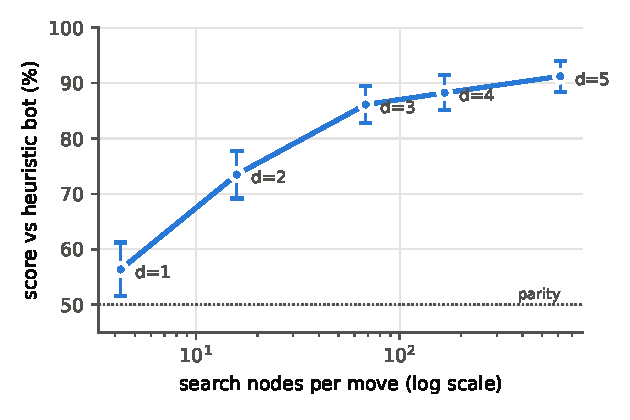
\includegraphics[width=0.62\linewidth]{report/figures/minimax_depth.pdf}
\caption{Strength vs.\ search cost for minimax depths 1--5 on \bx{6}. Error bars:
95\% CI.}
\label{fig:depth}
\end{figure}

Table~\ref{tab:depth} and Fig.~\ref{fig:depth} show strength rising
monotonically with depth, with clearly diminishing returns per node. The first
two extra plies give most of the gain, and later plies each cost several times
more search for a smaller improvement. Depth~1 is a useful internal check. A
one-ply search with the same evaluation \emph{is} the greedy heuristic bot. It
scores only slightly above parity, and we attribute the residual edge to the
opponent's $\varepsilon$-random moves.

We attribute the early gains to the \emph{horizon effect}: an evaluation is
blind to consequences that fall just beyond its search depth. A greedy bot
cannot see that a move gives the opponent a corner on the very next turn, and a
two- or three-ply search can. Once that blunder class is covered, extra depth
only refines decisions that the evaluation already ranks reasonably, and the
gains flatten.

The effective branching factor alternates between larger and smaller values from
one depth to the next rather than staying constant. We hypothesise this is
alpha-beta's \emph{odd-even effect}: pruning efficiency differs depending on
whether the last ply belongs to the searching side or its opponent. We have not
verified this with a separate experiment.

We keep \textbf{depth 4} as the reference minimax. It sits after the steep part
of the curve, and depth~5 costs several times more per game. This matters
because minimax will be evaluated thousands of times during RL training.

\subsection{Head-to-head comparison}
\label{sec:bots_compare}

The opponents must form a clear strength ladder before any RL result can be
interpreted. We originally required that heuristic beat random in at least 95\%
of games and that minimax-d4 beat heuristic in at least 80\%. The full round
robin was played on all three board sizes with the weights tuned on \bx{6}.

The minimax criterion passed easily at every size. The heuristic criterion
\emph{failed at every size}. On \bx{6} the 95\% confidence interval lies wholly
below the bar, so this was a real shortfall, not sampling noise. The two
diagnostics below look for the cause. The resulting, revised gate is
reported in Table~\ref{tab:gate}.

\begin{table}[H]
\centering
\caption{Diagnostic: win rate (\%) and mean disc margin against the random bot
for variants of the heuristic bot (6-ply random openings).}
\label{tab:diag}
\begin{tabular}{@{}lrrrr@{}}
\toprule
& \multicolumn{2}{c}{\bx{6} (1000 games)} & \multicolumn{2}{c}{\bx{8} (400 games)} \\
\cmidrule(lr){2-3}\cmidrule(l){4-5}
Agent & Win & Margin & Win & Margin \\
\midrule
\tabinput{report/tables/gate_diag.tex}
\bottomrule
\end{tabular}
\end{table}

\begin{table}[H]
\centering
\caption{Diagnostic: heuristic vs.\ random on \bx{6} as a function of the number
of random opening plies (1000 games per row). ``Distinct'' counts the unique
openings among the 500 generated.}
\label{tab:openings}
\begin{tabular}{@{}rrrlrl@{}}
\toprule
& & \multicolumn{2}{c}{$\varepsilon=0.05$} & \multicolumn{2}{c}{$\varepsilon=0$} \\
\cmidrule(lr){3-4}\cmidrule(l){5-6}
Opening plies & Distinct & Win (\%) & Score (\%) & Win (\%) & Score (\%) \\
\midrule
\tabinput{report/tables/gate_openings.tex}
\bottomrule
\end{tabular}
\end{table}

We tested three candidate causes.
\begin{enumerate}[leftmargin=*]
  \item \textbf{Exploration noise.} Removing the $\varepsilon$-random moves
        helps only slightly (Tables~\ref{tab:diag} and~\ref{tab:openings}), so
        it is not the main cause. As expected, the greedy bot and minimax-d1
        perform the same, a second consistency check on the search code.
  \item \textbf{Opening luck.} A \bx{6} game lasts only about two dozen plies
        (Table~\ref{tab:throughput}), so six random opening plies are a
        substantial fraction of it. Table~\ref{tab:openings} supports this
        \emph{partially}. Fewer random plies raise the win rate, but only
        modestly, and the rate stays below 95\% even from the plain start
        position. Short openings also collapse diversity: two plies give only
        about a dozen distinct openings.
  \item \textbf{Myopia (horizon effect).} This is the remaining and, we infer,
        dominant cause. A one-ply evaluation cannot see the opponent's reply,
        so even a random opponent is sometimes handed a corner. Lookahead is the
        only change that substantially closes the gap: depth~2 nearly reaches
        the bar on \bx{6} and clears it comfortably on \bx{8}
        (Table~\ref{tab:diag}).
\end{enumerate}
\bx{6} has the largest gap of the three sizes. We attribute this to the short
game, which limits the number of decisions in which the better player can pull
ahead.

\paragraph{Resolution.} A greedy one-ply bot cannot reliably reach 95\% against
random on \bx{6}. The 95\% bar was a prior guess, not a property of the game.
We therefore revised the heuristic criterion to a \textbf{score of at least
90\%} (draws count half). For consistency the minimax criterion is also stated
on score. We kept the 6-ply openings because evaluation diversity matters more
to the later studies than a few points of heuristic strength. We rejected
replacing the heuristic bot with minimax-d2. A weaker-but-solid training
opponent leaves more headroom for the learning curves in
\S\ref{sec:classical}, and minimax-d4 already provides the strong reference.

\flag{\textbf{This threshold was chosen after seeing the data.} On \bx{6} the
heuristic bot clears the revised bar on score only narrowly. Its raw win rate
is just below 90\%, because draws are frequent on the small board. Read the
heuristic--random gap as ``clear and stable'', not ``overwhelming''.}

\begin{table}[H]
\centering
\caption{Round robin between the reference opponents. Wins/draws/losses,
win rate and score are from the first-named agent's perspective. Games $=2\times$
openings. Gate: the revised threshold on \emph{score} and its outcome.}
\label{tab:gate}
\small
\begin{tabular}{@{}llrcrlrl@{}}
\toprule
Board & Match-up & Games & W/D/L & Win (\%) & Score (\%) & Margin & Gate \\
\midrule
\tabinput{report/tables/gate.tex}
\bottomrule
\end{tabular}
\end{table}

\begin{figure}[H]
\centering
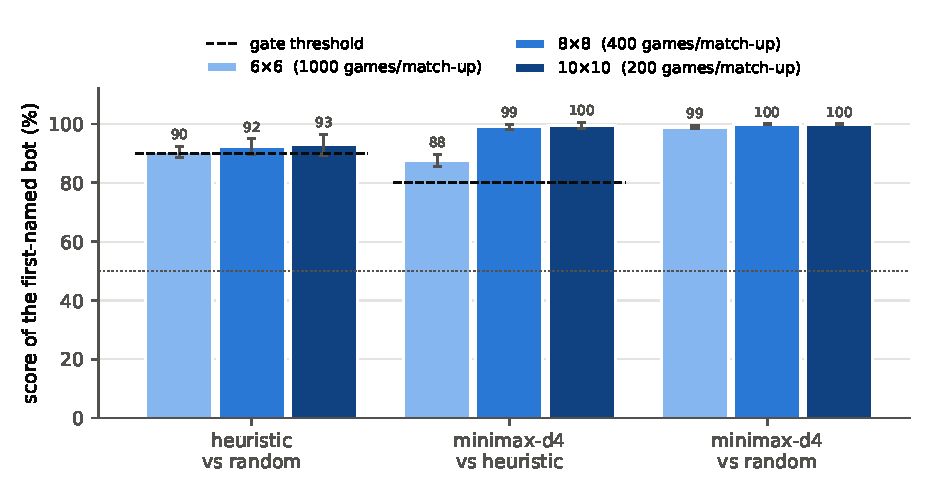
\includegraphics[width=\linewidth]{report/figures/bots_head_to_head.pdf}
\caption{Head-to-head comparison of the three rule-based bots on each board
size. Each bar is the score of the first-named (stronger) bot. Whiskers: 95\% CI;
dashed segments: gate thresholds; dotted line: 50\% (parity). The \bx{6}-tuned weights of
the heuristic were used on every size.}
\label{fig:bots_h2h}
\end{figure}

\subsection{Elo ratings}
\label{sec:elo}

Win rates describe one pairing at a time. An \emph{Elo rating}
\cite{elo1978} puts every player on a single numeric scale, so that the
difference between two ratings predicts the result of a match between them.
Under the Elo model a player rated $\Delta$ points above an opponent is expected
to score
\[
  E(\Delta) \;=\; \frac{1}{1 + 10^{-\Delta/400}} ,
\]
where a score counts a win as 1 and a draw as $\tfrac12$. The constant 400 sets
the units. A gap of 0 means an even match, 100 points means an expected score of
about 64\%, 200 points about 76\%, 400 points about 91\% and 800 points about
99\%. Only differences between ratings carry meaning. We therefore fix the
random bot at 0, so every other rating reads as ``points above random play''.

\paragraph{How the ratings are fitted.} Chess federations update Elo
incrementally after each game. Here every game is already played, so we fit all
ratings at once with the \emph{Bradley--Terry} model \cite{bradley1952}, the
statistical model behind Elo. It gives each player a strength $\gamma_i>0$ and
models the probability that $i$ beats $j$ as $\gamma_i/(\gamma_i+\gamma_j)$,
which is exactly $E(\Delta)$ with rating $R_i = 400\log_{10}\gamma_i$. The
strengths are the maximum-likelihood fit to the full round robin. They are
computed with the minorisation--maximisation algorithm of \cite{hunter2004},
with draws counting as half a win for each side
(\texttt{othello/eval/elo.py}). If a player never loses, the maximum-likelihood
rating is infinite. A weak prior, one virtual drawn game against a reference
opponent, keeps such ratings finite.

\paragraph{Why a single scale is useful.} The ratings compress the round robin
into one ordering with interpretable gaps. They also make strength
\emph{comparable across opponents}: any agent that plays the reference bots can
be placed on the same scale, including the learning agents of later sections.

\begin{table}[H]
\centering
\caption{Elo ratings of the three rule-based bots, fitted separately to each
size's round robin (random $=0$; \S\ref{sec:elo}). Near-perfect scores make the
larger gaps poorly determined; a weak prior keeps them finite.}
\label{tab:elo}
\begin{tabular}{@{}lrrr@{}}
\toprule
Board & random & heuristic & minimax-d4 \\
\midrule
\tabinput{report/tables/elo.tex}
\bottomrule
\end{tabular}
\end{table}

\begin{table}[H]
\centering
\caption{Consistency check of the Elo scale. ``Gap'' is the rating difference
from Table~\ref{tab:elo}, ``Predicted'' is the score $E(\text{gap})$ it implies,
and ``Observed'' is the measured score with its 95\% CI (Table~\ref{tab:gate}).}
\label{tab:elo_check}
\small
\begin{tabular}{@{}llrrl@{}}
\toprule
Board & Match-up & Gap & Predicted (\%) & Observed (\%) \\
\midrule
\tabinput{report/tables/elo_check.tex}
\bottomrule
\end{tabular}
\end{table}

\paragraph{Is one scale enough?} A rating scale is only meaningful if strength
is \emph{transitive}: if A beats B and B beats C, A must beat C by at least as
much. Games need not behave this way, since strategies can cycle like
rock--paper--scissors. With three players and three pairings the model has only
two free gaps for three observed scores, so the fit can fail. In
Table~\ref{tab:elo_check}, every predicted score falls inside the confidence
interval of the observed one, on every board size. In particular, the gaps add
up: the minimax--random gap is the sum of the other two and still predicts its
pairing. The three bots therefore lie on a single, consistent strength line.

\paragraph{Limitations.} Where a bot almost never loses, as minimax-d4 does on
\bx{8} and \bx{10}, the data only say that the gap is \emph{large}. The rating
is then set mostly by the prior, and is best read as a lower bound. Ratings are
also relative to this pool and protocol: they are not comparable with human or
engine Elo ratings measured elsewhere. Finally, the scale assumes strength is
one-dimensional. An agent that exploits one particular opponent, like the Monte
Carlo learner of \S\ref{sec:classical}, would fit poorly, and the fit's
residuals would show it.

Fig.~\ref{fig:bots_h2h} and Tables~\ref{tab:gate} and~\ref{tab:elo} confirm the intended ordering
random $<$ heuristic $<$ minimax on every board size. The gap between minimax
and heuristic widens as the board grows. We attribute this to two effects.
Larger boards mean longer games with more decisions, so lookahead has more
chances to pay off. And the weights were tuned on \bx{6}, which likely suits the
greedy bot less on bigger boards, while search partly makes up for a mis-tuned
evaluation.

%======================================================================
\section{Traditional Training Methods}
\label{sec:classical}

This section trains five classical RL methods on \bx{6}. All of them use the
same fixed opponent and the same budget, and each is then compared against all
three rule-based bots. The question is not only how well each method plays, but
\emph{why} it stops improving where it does.

\subsection{Common setup}
\begin{itemize}[leftmargin=*]
  \item \textbf{Opponent and episodes.} Each learner plays the heuristic bot
        (\S\ref{sec:bots}), alternating colours and starting from random
        6-ply openings, for \TrainGames{} training games per run, with 3 seeds
        per method.
  \item \textbf{The learner's view.} The learner sees only its own decision
        points. Its state $s_t$ is the position when it is to move, and the
        opponent's reply is part of the environment's transition to $s_{t+1}$.
        The reward is $+1$, $0$ or $-1$ at the end of the game and zero
        otherwise, with no discounting ($\gamma=1$).
  \item \textbf{Exploration.} $\varepsilon$-greedy, with $\varepsilon$ decaying
        linearly from 0.3 to 0.05 over the first half of training.
  \item \textbf{Evaluation.} Every 5{,}000 games the greedy policy plays 200
        evaluation games against the heuristic bot (for the learning curves).
        At the end it plays 1{,}000 games against random and against heuristic,
        and 500 against minimax-d4 (for the comparison). The evaluation
        openings are fixed and shared across methods.
\end{itemize}

\subsection{The methods}

\paragraph{Tabular Q-learning \cite{watkins1992}.} Keeps a table entry $Q(s,a)$
for every state--action pair it has visited and updates it toward a bootstrapped
one-step target:
\[
  Q(s_t,a_t) \leftarrow Q(s_t,a_t) + \alpha\big[r_{t+1} + \gamma \max_{a'} Q(s_{t+1},a') - Q(s_t,a_t)\big].
\]
The $\max$ makes it \emph{off-policy}: it learns the value of the greedy policy
while it behaves $\varepsilon$-greedily. To give the table its best chance, each
position is stored in a canonical form under the 8 symmetries of the board, so
symmetric positions share one entry. Unvisited entries read as 0.

\paragraph{SARSA \cite{rummery1994}.} Identical to Q-learning except that the
target uses the action $a_{t+1}$ the agent \emph{actually} took next, i.e.
$r_{t+1} + \gamma Q(s_{t+1},a_{t+1})$. It is therefore \emph{on-policy}: it values
the exploring policy itself, including its exploratory mistakes.

\paragraph{First-visit Monte Carlo control \cite{sutton2018}.} Does not
bootstrap. After the game ends, every visited pair is moved toward the observed
return $G_t$ (here the final result) by a sample average,
$Q(s,a)\leftarrow Q(s,a) + \tfrac{1}{N(s,a)}\,[G_t - Q(s,a)]$. Its targets are
unbiased but have high \emph{variance}: each one is a single noisy game outcome
that depends on every later move by both players. (Positions never repeat within
an Othello game, so first-visit and every-visit MC coincide.)

\paragraph{Linear function-approximation Q-learning.} Replaces the table with a
weighted sum of features, $Q(s,a)=\mathbf{w}^{\top}\boldsymbol{\phi}(s\!\oplus\!a)$,
where $s\!\oplus\!a$ is the \emph{afterstate}: the position right after the
learner's move. The features are disc difference, mobility difference, corner
difference, X-square difference, stable-edge-disc difference and a bias, each
scaled to roughly unit range. The weights are learned by semi-gradient
Q-learning, $\mathbf{w} \leftarrow \mathbf{w} + \alpha\,\delta_t\,\boldsymbol{\phi}$.
Unlike a table, it \emph{generalises}: every position with similar features gets a
similar value, even if it has never been seen. But it can only represent
evaluations that are linear in those features.

\paragraph{Vanilla DQN \cite{mnih2015}.} Replaces the table with a neural network
$Q_\theta$: an MLP with two hidden layers of 256 units over three input planes
(own discs, opponent discs, legal moves). It outputs one value per square plus
pass. Two components stabilise training:
an \emph{experience-replay} buffer (200k transitions, sampled uniformly), which
breaks the correlation between consecutive positions, and a \emph{target
network} $Q_{\theta^-}$, synced every 2{,}000 updates, which keeps the bootstrap
target from chasing itself. The loss is
$\mathrm{Huber}\big(Q_\theta(s,a) - [r + \gamma\max_{a'\,\text{legal}} Q_{\theta^-}(s',a')]\big)$.
Illegal actions are masked both when acting and in the max. Unlike the linear
model, the network can learn its own features from raw discs.

\paragraph{Disc-count ablation (linear FA).} To test the disc-count trap
(\S\ref{sec:concepts}) on a learner, the linear method is trained three more
ways: without the disc feature, with \emph{only} the disc feature (plus bias),
and with the full feature set but rewarded by the final \emph{disc margin}
instead of win/loss.

\subsection{Results}
\label{sec:classical_results}
\subsubsection{Comparison against the three rule-based bots}

\begin{figure}[H]
\centering
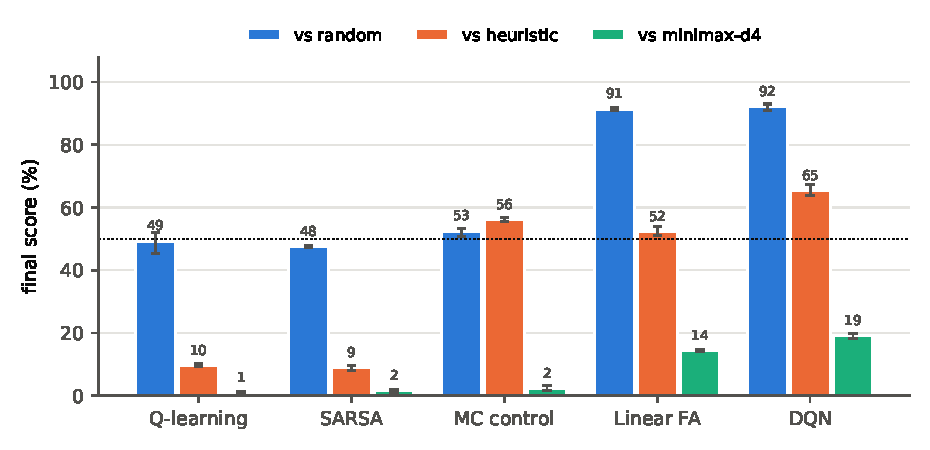
\includegraphics[width=\linewidth]{report/figures/classical_bars.pdf}
\caption{Final score of each traditional method against the three rule-based
bots on \bx{6}. Bars: mean over 3 seeds; whiskers: min--max across seeds; dotted
line: 50\% (parity). Against random and heuristic each bar is 1{,}000 games per
seed; against minimax-d4 it is 500.}
\label{fig:classical_bars}
\end{figure}

\begin{table}[H]
\centering
\caption{Final evaluation of the traditional methods (mean $\pm$ std over
seeds, \%). ``Win vs heur.'' is the raw win rate against the training opponent.
``Train'' is the wall-clock hours per run on one CPU core. The reference row is
the heuristic bot's own result from the rule-based round robin
(Table~\ref{tab:gate}). Bold: best per column.}
\label{tab:classical}
\small
\begin{tabular}{@{}lcllllr@{}}
\toprule
& & \multicolumn{3}{c}{Score vs.\ (\%)} & & \\
\cmidrule(lr){3-5}
Method & Seeds & random & heuristic & minimax-d4 & Win vs heur. & Train (h) \\
\midrule
\tabinput{report/tables/classical.tex}
\bottomrule
\end{tabular}
\end{table}

Figure~\ref{fig:classical_bars} and Table~\ref{tab:classical} separate the
methods into three tiers. The tabular TD methods (Q-learning and SARSA) never
leave random play: they draw level with the random bot and lose almost every game
to the other two. Linear function approximation reaches the strength of the
heuristic bot: it scores about as well as the heuristic does against random,
breaks even against the heuristic, and loses to minimax-d4 by a similar margin.
DQN is the strongest method on \emph{all three} opponents, and is the only one
that clearly beats its training opponent while still dominating random play.

Monte Carlo control does not fit this ordering. It beats the heuristic bot it was
trained against, yet against the \emph{random} bot it does no better than a coin
flip. A policy that had learned to play Othello would find the random bot the
easiest of the three opponents. MC control instead does well only against the
one opponent it has seen. We call this \emph{overfitting to the training
opponent}: a policy that exploits the specific habits of one opponent instead of
learning the game. Evaluating against the training opponent alone would have
ranked MC control among the best methods. The three-bot comparison is what
exposes it. No method comes close to minimax-d4. Every one of them chooses moves
without lookahead, and none overcomes the horizon effect that already limited
the one-ply heuristic bot (\S\ref{sec:bots}).

\subsubsection{Learning dynamics}

\begin{figure}[H]
\centering
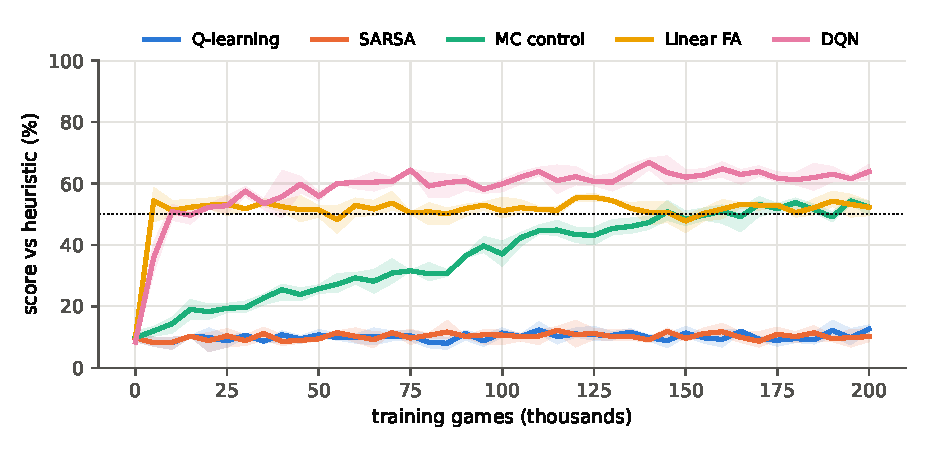
\includegraphics[width=\linewidth]{report/figures/classical_curves.pdf}
\caption{Learning curves: greedy-policy score against the heuristic bot (200
games per point) during training. Lines: mean over 3 seeds; bands: min--max.
Q-learning and SARSA overlap almost exactly.}
\label{fig:classical_curves}
\end{figure}

The curves in Fig.~\ref{fig:classical_curves} show three different failure modes.

\begin{itemize}[leftmargin=*]
  \item \textbf{Flat at the bottom (Q-learning, SARSA).} No measurable
        improvement over the whole budget.
  \item \textbf{Immediate plateau (linear FA).} Reaches parity within the first
        evaluation interval and then does not move. Additional data does not
        help.
  \item \textbf{Slow, steady climb (MC control, DQN).} Both are still rising
        at the end of the budget, MC control from a much lower start.
\end{itemize}

\subsubsection{Why the tabular methods fail}

\begin{table}[H]
\centering
\caption{Tabular diagnostics at the end of training (mean over 3 seeds).
Coverage is the fraction of the learner's decision positions during the final
evaluation games that already have an entry in its table. Update-error variance
is the variance of $(\text{target} - Q)$ over the updates of the first and of the
last 5{,}000 training games.}
\label{tab:tabular}
\small
\begin{tabular}{@{}lrrrrr@{}}
\toprule
& & \multicolumn{2}{c}{Coverage (\%)} & \multicolumn{2}{c}{Update-error var.} \\
\cmidrule(lr){3-4}\cmidrule(l){5-6}
Method & States ($10^6$) & vs heuristic & vs random & first 5k & last 5k \\
\midrule
\tabinput{report/tables/classical_tabular.tex}
\bottomrule
\end{tabular}
\end{table}

\paragraph{The curse of dimensionality.} Table~\ref{tab:tabular} shows the
mechanism directly. After \TrainGames{} games each table holds between one and two million
canonical positions, yet in games against the random bot fewer than one in ten
of the positions the learner meets are in its table. A lookup table has no notion of
similarity between positions, so a position it has not seen is a position it
knows nothing about, and it falls back to an arbitrary choice. This is the
\emph{curse of dimensionality} in its plainest form: the number of reachable
positions is so large that a table cannot be filled from any feasible amount of
play. It is the same even after merging the 8 board symmetries. Coverage is
markedly higher against the heuristic bot, because a mostly deterministic
opponent keeps leading the game back into the same lines. That difference is
what MC control exploits.

\paragraph{Why Q-learning and SARSA are indistinguishable.} The two update rules
differ only in which next-state entry they bootstrap from: the greedy one or the
one actually taken. A unit test confirms they produce different targets when the
next state's entries exist (\texttt{tests/test\_rl.py}). In practice the next
state is usually unvisited, so both entries read the default value of zero, the
two targets coincide and the learners behave the same. We attribute the TD
methods' failure to
\emph{bootstrapping} under sparse revisits. A one-step target $r+\gamma
Q(s',\cdot)$ only carries information backwards one move per visit. The final
reward therefore has to travel back through many revisits of the same line before
it reaches early positions, and almost no line is revisited that often.

\paragraph{Why MC control behaves differently.} MC control does not bootstrap.
After every game it moves \emph{all} visited entries straight toward the actual
outcome, so a single winning game against the heuristic bot marks every position
on that line as good at once. Against a nearly deterministic opponent, starting
from a bounded set of openings, the same lines come back often enough for these
marks to accumulate. Its coverage against the heuristic bot rises together with
its score. It is effectively memorising a growing book of winning lines against
\emph{that one bot}. Coverage against the random bot stays low, which is why the
memorised book is useless there. The price of not bootstrapping is
\emph{variance}. Each MC target is a single, noisy game outcome, and its
update-error variance is several times that of the TD methods. That variance is
the bias--variance trade-off in action: unbiased targets, but slow and noisy
progress, consistent with its slow climb in Fig.~\ref{fig:classical_curves}.

\flag{\textbf{Design note.} We added the heuristic bot's $\varepsilon$-randomness
and the random openings specifically to stop a tabular learner from memorising
lines against it (\S\ref{sec:bots}). This was \emph{not sufficient}. MC control
still found enough repetition to exploit. Any future result measured only
against the training opponent should be treated with suspicion. The curve
was still rising at the end of the budget, and we expect, but have not tested,
that longer training would increase this exploitation without improving play
against other opponents.}

\subsubsection{Why linear function approximation plateaus}
The linear learner \emph{generalises}: two positions with similar features get
similar values whether or not either was seen. That is why it beats the random
bot as convincingly as the heuristic bot does, after almost no training. But it
reaches its ceiling almost immediately and stays there. Its features are
essentially the heuristic bot's own features plus edge stability, so the best
policy it can represent is a re-weighted one-ply heuristic. Learning finds those
weights within a few thousand games, and the learned weights reproduce the
ordering found by the weight search (\appref{app:heuristic}): corners first, then mobility, with disc count near
zero (Table~\ref{tab:ablation}). This is a \emph{capacity} or
\emph{inductive-bias} limit rather than a data limit. The model class itself
contains nothing better than the heuristic, so more games cannot help.

\subsubsection{Why DQN is the strongest, and still loses to search}
DQN combines the two missing ingredients. It generalises across positions like
the linear model, but it learns its own features from raw disc planes instead of
being restricted to hand-chosen ones. Replay lets each game be learned from many
times, and the target network keeps the bootstrapped targets stable while it
does. The result is the only method that improves on the heuristic bot without
losing generality. It still chooses each move from a single forward pass, with no
lookahead. Minimax-d4 punishes exactly the tactical oversights a one-ply policy
cannot see, which is why DQN loses heavily to it. Its curve is still rising, so a
longer run would likely help somewhat. However, closing the gap to search is the
job of the self-play and MCTS methods in \S\ref{sec:next}, not of more DQN
training.

\subsubsection{The disc-count ablation}

\begin{figure}[H]
\centering
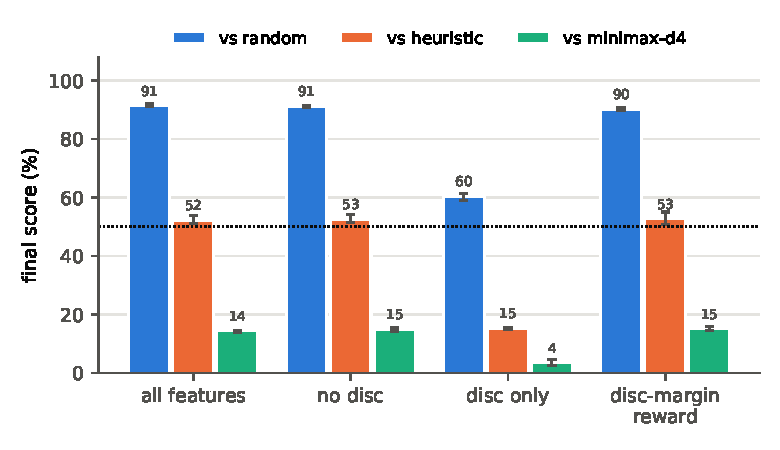
\includegraphics[width=0.8\linewidth]{report/figures/classical_ablation_bars.pdf}
\caption{Disc-count ablation for linear function approximation. Same format as
Fig.~\ref{fig:classical_bars}.}
\label{fig:ablation}
\end{figure}

\begin{table}[H]
\centering
\caption{Disc-count ablation (mean $\pm$ std over 3 seeds, \%), with the learned
weights (mean over seeds) on the scaled disc, mobility and corner features.}
\label{tab:ablation}
\small
\begin{tabular}{@{}llllrrr@{}}
\toprule
& \multicolumn{3}{c}{Score vs.\ (\%)} & \multicolumn{3}{c}{Learned weight} \\
\cmidrule(lr){2-4}\cmidrule(l){5-7}
Variant & random & heuristic & minimax-d4 & disc & mob. & corner \\
\midrule
\tabinput{report/tables/classical_ablation.tex}
\bottomrule
\end{tabular}
\end{table}

Fig.~\ref{fig:ablation} and Table~\ref{tab:ablation} separate two versions of
the disc-count trap.
\begin{itemize}[leftmargin=*]
  \item \textbf{Disc-count \emph{features}: the trap is reproduced.} Removing
        the disc feature changes nothing, and the full model learns to give it
        essentially zero weight. A learner restricted to disc count \emph{only}
        collapses to the strength of the disc-greedy bot from the tuning study
        (\appref{app:heuristic}),
        barely above random. Disc count simply does not carry the information
        needed to play well. The learner rediscovers what the rule-based
        tuning found (\appref{app:heuristic}).
  \item \textbf{Disc-count \emph{reward}: no measurable harm.} Rewarding the
        final disc margin instead of the win leaves strength unchanged on all
        three opponents. This \emph{contradicts} the expectation in our original
        plan. We attribute it to the features. With corner and mobility features
        available, the positions that maximise the final margin are the same
        ones that maximise the chance of winning, so the two objectives agree.
        The learned weights only shrink in scale, as the smaller reward range
        would predict, and keep their ordering. The trap lies in valuing discs
        \emph{during} the game, which the features control, not in scoring them
        at the \emph{end}, which is all the reward does.
\end{itemize}

%======================================================================
\section{Self-Play Methods}
\label{sec:selfplay}

Every method in \S\ref{sec:classical} learned by playing the heuristic bot, so
it could at best learn to beat \emph{that} bot. In \emph{self-play} the learner
plays against itself, or against frozen copies of its earlier selves. The
opponent therefore improves as the learner does, and no hand-written opponent
is needed during training. This section compares three self-play methods on
\bx{6}. The evaluation is unchanged: the same three rule-based bots, openings
and protocol as before. The heuristic bot is now used \emph{only} for
evaluation and is never trained against. The strongest agent becomes the
project's final model, \textit{Oroletto}.

\subsection{The methods}

\paragraph{DQN+ (Double DQN with an opponent pool).} The DQN of
\S\ref{sec:classical} with two changes. First, the bootstrap target is a
\emph{Double DQN} target \cite{vanhasselt2016},
$r + \gamma\,Q_{\theta^-}\!\big(s',\arg\max_{a'} Q_\theta(s',a')\big)$: the online
network picks the next action and the target network scores it. This removes
the systematic over-estimation that comes from taking a max over noisy
estimates. Second, the opponent is drawn from an \emph{opponent pool}. Every
5{,}000 games a frozen snapshot of the learner joins the pool (at most 20 kept),
and each training game is played against the live learner with probability
$\tfrac12$, otherwise against a random snapshot. Playing past selves protects
against \emph{strategy cycling}, where a learner that only ever plays its latest
self forgets how to beat strategies it has already moved past.

\paragraph{Self-play PPO.} Proximal Policy Optimisation \cite{schulman2017} learns
a policy $\pi_\theta(a\mid s)$ and a value $V_\theta(s)$ directly. Here an MLP
with a shared trunk, a masked softmax over legal moves and a $\tanh$ value head
is used. Experience is collected from complete games, 4{,}096 learner decisions
per update, with advantages $\hat A_t$ from generalised advantage estimation
($\lambda=0.95$). The policy is improved with the \emph{clipped} objective
\[
  \mathcal{L}^{\text{clip}} = \mathbb{E}_t\Big[\min\big(\rho_t \hat A_t,\;
  \mathrm{clip}(\rho_t, 1-\epsilon, 1+\epsilon)\,\hat A_t\big)\Big],\qquad
  \rho_t = \frac{\pi_\theta(a_t\mid s_t)}{\pi_{\text{old}}(a_t\mid s_t)},
\]
with $\epsilon = 0.2$. Clipping keeps each update close to the policy that
collected the data, which is what makes reusing a batch for several epochs
safe. PPO uses the same opponent pool as DQN+, and only the learner's own moves
are used for updates, so the data stay on-policy.

\paragraph{AlphaZero.} Following \cite{silver2018}, a single residual network
$f_\theta(s) = (\mathbf{p}, v)$ outputs a move distribution $\mathbf{p}$ and a value
$v\in[-1,1]$. It has 4 residual blocks of 64 channels (about 0.3\,M parameters),
and its input planes are own discs, opponent discs and legal moves. Moves are
chosen by \emph{Monte Carlo tree search} (MCTS) guided by the network. Each of
the 64 simulations per move descends the tree by the PUCT rule
\[
  a^\ast = \arg\max_a \Big[\, Q(s,a) + c_{\text{puct}}\, P(s,a)\,
  \frac{\sqrt{N(s)}}{1+N(s,a)} \Big],
\]
where $Q$ is the mean value of the simulations through $(s,a)$, $P$ the network's
prior, $N$ visit counts and $c_{\text{puct}}=1.5$. The leaf is evaluated by the
network rather than by a random rollout. In self-play, Dirichlet noise is mixed
into the root priors, and the first 10 plies are sampled in proportion to visit
counts to diversify the games; after that the most-visited move is played. Each
position stores its visit distribution $\boldsymbol{\pi}$ and the final result
$z$. The network is trained on a sliding window of the latest 150{,}000 positions
to minimise
\[
  \mathcal{L} = (z - v)^2 \;-\; \boldsymbol{\pi}^{\top}\log \mathbf{p} \;+\; c\,\lVert\theta\rVert^2 ,
\]
and each batch is transformed by a random one of the 8 board symmetries. The key
idea is that \emph{search acts as a policy-improvement operator}. MCTS with the
current network plays better than the network alone, and the network is then
trained to imitate the search. The next search starts from a better prior, and
so on.

\paragraph{Budgets.} DQN+ and PPO play 200{,}000 self-play games, like the
classical methods. AlphaZero plays 100{,}000. One AlphaZero game costs far more
compute, because every move runs 64 network-guided simulations. Each method
uses 3 seeds. Wall-clock times are reported alongside game counts.

\subsection{Results}

\begin{figure}[H]
\centering
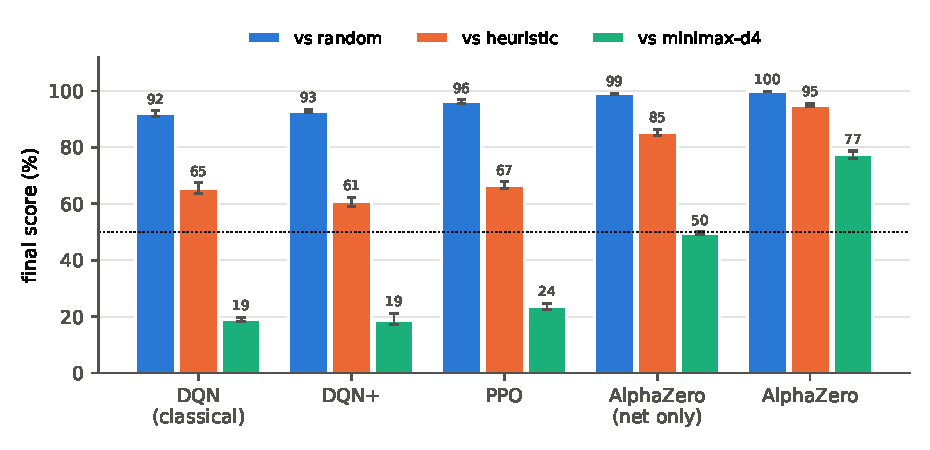
\includegraphics[width=\linewidth]{report/figures/selfplay_bars.pdf}
\caption{Final score of the self-play methods against the three rule-based
bots on \bx{6}, with classical DQN (\S\ref{sec:classical}) for reference. Bars:
mean over 3 seeds; whiskers: min--max; dotted line: 50\%. ``AlphaZero (net
only)'' plays the trained network's top move with no search; ``AlphaZero''
searches 64 simulations per move.}
\label{fig:selfplay_bars}
\end{figure}

\begin{table}[H]
\centering
\caption{Self-play methods compared (mean $\pm$ std over 3 seeds). ``Games to
60/80\%'' is the number of training games after which the score against the
heuristic bot first reaches that level (mean over seeds; evaluated every
5{,}000 games, so $\le$5k means ``by the first checkpoint''; -- means never).
Train: wall-clock hours per run.}
\label{tab:selfplay}
\small
\begin{tabular}{@{}lclllrrrr@{}}
\toprule
& & \multicolumn{3}{c}{Final score vs.\ (\%)} & \multicolumn{2}{c}{Games to} & & \\
\cmidrule(lr){3-5}\cmidrule(lr){6-7}
Method & Seeds & random & heuristic & minimax-d4 & 60\% & 80\% & Games & Train (h) \\
\midrule
\tabinput{report/tables/selfplay.tex}
\bottomrule
\end{tabular}
\end{table}

\begin{figure}[H]
\centering
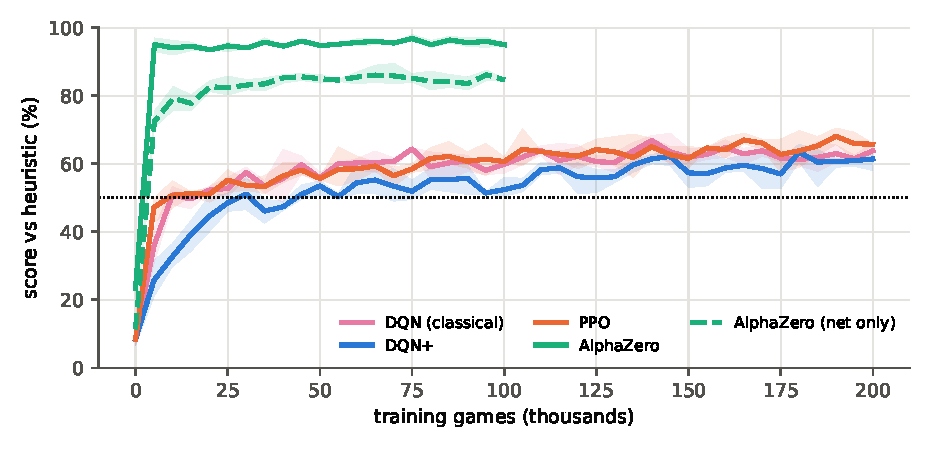
\includegraphics[width=\linewidth]{report/figures/selfplay_curves.pdf}
\caption{Learning curves: score against the heuristic bot during training (200
games per point; mean over 3 seeds, band: min--max). Only classical DQN trains
against this bot; the others never see it during training.}
\label{fig:selfplay_curves}
\end{figure}

Fig.~\ref{fig:selfplay_bars} and Table~\ref{tab:selfplay} show a single, very
large gap. DQN+ and PPO land at the level of classical DQN. AlphaZero is far
above all of them on every opponent. It wins almost every game against the
heuristic bot, and it is the first agent in this project that clearly beats
minimax-d4.

\paragraph{Self-play without search: as good as the best fixed-opponent
learner.} DQN+ and PPO reach the strength of classical DQN without ever playing
the heuristic bot, and PPO is slightly ahead on all three opponents. Self-play
therefore removes the need for a hand-written training opponent at no cost in
strength. It also removes the failure mode of \S\ref{sec:classical}: no
self-play learner shows the ``beats its training opponent but not random''
pattern of Monte Carlo control. Their curves (Fig.~\ref{fig:selfplay_curves})
are still rising slowly at the end, as classical DQN's was. They level off near
the same score, against heuristic and against minimax alike. We attribute this
shared ceiling to what all three have in common: a one-step-lookahead policy
computed by an MLP, with no search at play time. DQN+ learns more slowly than
PPO. We hypothesise that the over-estimation fix and the opponent pool help
less than PPO's direct policy updates when the reward is a single game result,
but we have not tested this.

\paragraph{AlphaZero: two distinct contributions of search.} The two AlphaZero
bars separate two roles of search.
\begin{itemize}[leftmargin=*]
  \item \textbf{Search at play time.} The same network gains substantially,
        most of all against minimax-d4, when it is allowed to search 64
        simulations per move. Search does at play time what minimax does: it
        looks at replies, which removes the horizon blunders that cap every
        one-ply policy.
  \item \textbf{Search as a training signal.} Even \emph{without} search, the
        AlphaZero network is far stronger than the DQN+ or PPO networks. It
        draws level with minimax-d4 where they score about one in five. Its
        targets are what makes the difference. It is trained to imitate MCTS
        visit counts, a policy already improved by lookahead, rather than to
        fit noisy game outcomes one move at a time.
\end{itemize}
One confound remains. The AlphaZero network is a convolutional residual
network, while DQN+ and PPO use MLPs, so part of the second gap may come from
the architecture's spatial inductive bias rather than from the training signal.
The architecture sweep in \S\ref{sec:next} is designed to separate the two.

\paragraph{Sample efficiency and compute.} AlphaZero passes 80\% against the
heuristic bot by its first checkpoint, and its network alone does so within
15{,}000 games. DQN+ and PPO never reach 80\%. Per game, however, AlphaZero is
much more expensive: each move runs 64 network-guided simulations, and a run took
several times longer in wall-clock time than a PPO run with twice as many games.
The comparison still favours AlphaZero clearly. It reached 80\% at its first checkpoint, after
under twenty minutes of training, a level PPO did not reach in its full run.

\paragraph{Stability.} Seed-to-seed spread is small for every method
(Table~\ref{tab:selfplay}), so the gaps between methods are far larger than
the noise.

\flag{\textbf{Limitation: the training curve saturates.} AlphaZero's score
against the heuristic bot levels off near 95\% after roughly 20{,}000 games
(Fig.~\ref{fig:selfplay_curves}). After that point the curve can no longer show
progress. Minimax-d4, the only opponent still able to separate strong agents,
was played only at the end, and intermediate checkpoints were not kept. We
therefore cannot say whether AlphaZero was still improving in the second half
of training. Future runs should save checkpoints and track a stronger
yardstick, such as minimax at depth 6, throughout.}

\subsection{Comparison with the solved game}

\begin{table}[H]
\centering
\caption{The final model playing itself from the standard \bx{6} start
position, with greedy MCTS at three search budgets (3 games each, different
seeds), compared with perfect play \cite{feinstein1993}. Results are Black--White
disc counts.}
\label{tab:solved}
\begin{tabular}{@{}rcll@{}}
\toprule
Simulations & Games & Result(s) & Winner \\
\midrule
\tabinput{report/tables/solved.tex}
\bottomrule
\end{tabular}
\end{table}

\bx{6} Othello is solved: with perfect play from the start, White wins 20--16
\cite{feinstein1993}. Our final model agrees on the \emph{winner}. Its value
head rates the start position at \StartValue{} from Black's side, a clear
prediction that Black loses. In self-play from the start, White wins every game
at every search budget (Table~\ref{tab:solved}). It does \emph{not} reproduce
the perfect-play \emph{margin}. White always wins by more than 4 discs. Perfect
play guarantees Black at least 16, so a wider margin proves that Black is
making mistakes. The model has learned which side is winning, but it does not
play perfectly. Self-play was also mostly trained from random openings rather
than from the start position, which may contribute.

\subsection{The final model: Oroletto}
\label{sec:oroletto}

The three AlphaZero seeds are within noise of each other. We chose the final
model by its score against the strongest opponent, minimax-d4, since the
weaker two opponents no longer separate the seeds. The selected run is
\texttt{results/alphazero/\OrolettoRun}, released as \textit{Oroletto} through
\texttt{models/oroletto.json}. Anyone can play it with
\texttt{othello --play oroletto}, which by default searches 200 simulations per
move, more than the 64 used in evaluation. We expect this to make it somewhat
stronger than the scores reported here, but we have not measured it.

%======================================================================
\section{System Architecture}
\label{sec:env}

All experiments run on one Python code base (package \texttt{othello}). It has
a size-parameterised environment, the bots, the learners, the evaluation
harness, and a terminal front-end for human play.

\subsection{Environment design}
\label{sec:arch}

The environment is shared by every experiment, and each part of it exists for
a downstream need:

\begin{description}[leftmargin=1.2em,style=nextline]
  \item[Bitboard state.] A position is two integers of $n^2$ bits (one per
  colour), plus the side to move and a consecutive-pass counter. Move
  generation shifts the bitboards in the eight compass directions and masks out
  bits that wrap around a row edge. Nothing depends on a fixed $n$, so \bx{6},
  \bx{8} and \bx{10} run the same code. This is the precondition for the
  size-generalisation study.
  \item[Immutable states.] Applying a move returns a new state rather than
  mutating the old one. Copying a position is therefore free, which tree
  search (minimax now, MCTS later) relies on to hold many positions at once.
  \item[Action space with an explicit pass.] Actions are the $n^2$ squares plus
  one \emph{pass} action. Pass is legal only when no placement is. A fixed-size
  action space with a legality mask lets learned policies mask illegal moves
  rather than learn to avoid them.
  \item[Configurable input planes.] The state can be encoded as any subset of
  \{own discs, opponent discs, empty squares, side to move, legal moves\}.
  The planned input-representation sweep (\S\ref{sec:next}) varies this set without
  touching the environment.
  \item[One agent interface.] Every player implements
  \texttt{act(state)$\to$action}. Bots, learned policies and search agents
  are therefore interchangeable in the evaluation harness.
\end{description}

\subsection{Evaluation protocol}
\label{sec:protocol}
All comparisons in this report use the same protocol. A fixed seed generates
$K$ opening positions by playing six uniformly random plies from the standard
start. Each opening is played twice with colours swapped, which cancels the
\emph{first-move advantage}: the systematic edge (positive or negative) that
comes from moving first rather than from playing well. Results are reported
from the first agent's perspective as wins/draws/losses, \emph{score}
(win $=1$, draw $=\tfrac12$) with a 95\% normal-approximation confidence
interval, and mean final disc margin. The random openings keep a deterministic
pair of agents from replaying one game $2K$ times. They also stop a learner from
memorising a single line against a fixed opponent, which matters for the
tabular methods in \S\ref{sec:classical}. Six plies give about 95\% distinct
openings at $K{=}500$, against about 42\% for four plies. The normal-approximation
interval degenerates (to zero width) when a score is exactly 0 or 1. Those
cells should be read as ``no losses observed'', not as certainty.

\subsection{Correctness validation}

\begin{table}[H]
\centering
\caption{Environment correctness checks (\NumTests{} automated tests, all passing; see
\texttt{results/baselines/pytest.txt}).}
\label{tab:tests}
\begin{tabularx}{\linewidth}{@{}lX@{}}
\toprule
Check & What it guards against \\
\midrule
Perft, \bx{8}, depth 1--6 & Errors in move generation or flipping. Leaf counts must equal the published values 4, 12, 56, 244, 1396, 8200. \\
Naive cross-check, $n\in\{4,6,8,10\}$ & Edge-wrapping errors at any board size. On 30 random games per size, the legal-move set and flipped discs must match an independent 2-D grid implementation at every ply. \\
Forced pass / double pass & Wrong termination. A player with no move must pass; two consecutive passes end the game; a placement resets the pass counter. \\
Full board, draw & Wrong winner attribution on equal disc counts. \\
Transpose symmetry & Direction-specific shift bugs. Transposing the board must transpose the legal-move set. \\
Encoding shapes & Plane-construction errors. Every plane configuration has shape $(C,n,n)$ with the expected disc and legal-move counts. \\
Agents & Illegal moves from any bot; minimax missing a forced win; the heuristic bot ignoring a corner. \\
\bottomrule
\end{tabularx}
\end{table}

Perft (``performance test'') counts the leaf positions of the full game tree to
a fixed depth. A single wrong flip or missed move changes the count, which makes
it the most sensitive check of the move generator. Perft only exists for
\bx{8}, so the naive cross-check carries the burden for the other sizes. It
compares the bitboard engine with an independent implementation that shares no
code with it, at every position of real games, including the board edges where
wrap-around bugs would appear.

\subsection{Simulator throughput}

\begin{table}[H]
\centering
\caption{Single-core simulator throughput, random vs.\ random, 1000 paired
openings per size. ``Black score'' is the share of points won by the first
mover under uniformly random play.}
\label{tab:throughput}
\begin{tabular}{@{}lrrrrr@{}}
\toprule
Board & Games & Games/s & Plies/s & Plies/game & Black score (\%) \\
\midrule
\tabinput{report/tables/throughput.tex}
\bottomrule
\end{tabular}
\end{table}

Table~\ref{tab:throughput} shows games per second falling steeply with board
size while plies per second fall only mildly. Almost all of the slowdown
therefore comes from games getting longer: the number of plies grows roughly with
the number of squares. Only a small part comes from each move costing more. Cost
per ply grows slowly because each bitboard operation acts on all $n^2$ squares
at once and the directional scans take $\mathcal{O}(n)$ steps. This tells us how
to budget compute. Simulation will be negligible next to neural-network
inference in the self-play studies, and going from \bx{6} to \bx{10} costs
mainly through game length. The pure-Python engine is therefore sufficient, and
a compiled engine is not needed yet.

On every board size the first mover scores slightly below half under random
play, so the side moving second has a small edge. This is \emph{consistent
with} the known result that \bx{6} Othello is a second-player win under
perfect play. Random play, however, says nothing about perfect play, so we
read it only as a reason to keep evaluating with both colours.

\subsection{Playing in the terminal}
\label{sec:cli}
The \texttt{othello} command lets a person play any agent in the terminal:
\texttt{othello --play [1--5 | beginner \dots expert]} chooses a rule-based bot,
\texttt{othello --model PATH} loads a trained model (linear or DQN),
\texttt{othello --play oroletto} plays \textit{Oroletto}, the project's final
trained model (\S\ref{sec:next}), and
\texttt{othello --tutorial} teaches the rules with the examples of
Fig.~\ref{fig:rules} before a coached practice game. Options cover the board size
(4--10), colour, legal-move hints and a coach mode that flags moves where the
expert bot disagrees. The command reuses the same environment and agent classes as
the experiments.

%======================================================================
\section{Next Steps}
\label{sec:next}

\begin{itemize}[leftmargin=*]
  \item \textbf{A stronger yardstick.} AlphaZero now beats minimax-d4 most of
        the time, so a stronger reference (minimax at depth 6 or more, or the
        Edax engine) is needed to keep measuring progress. Saving intermediate
        checkpoints would let learning curves be measured against it
        (\S\ref{sec:selfplay}). The same anchor would let every agent be placed
        on the Elo scale of \S\ref{sec:elo}.
  \item \textbf{Architecture and search-budget sweep.} Depth, width, input
        planes, head design and MCTS simulations, varied one at a time and
        summarised as a strength-versus-compute Pareto plot. This also separates
        the effect of AlphaZero's convolutional architecture from that of its
        search-based training signal (\S\ref{sec:selfplay}).
  \item \textbf{Scaling to \bx{8}.} Re-tune the rule-based bots for \bx{8}
        (Table~\ref{tab:gate} shows the \bx{6} weights are weaker there) and
        train the selected configuration. Optionally, play matches against the
        Edax engine.
  \item \textbf{One network for every board size.} Test zero-shot transfer,
        then train a fully convolutional, globally pooled network on mixed
        board sizes and compare it with a small-to-large curriculum. The result
        is reported as a train-size $\times$ test-size win-rate matrix.
\end{itemize}

%======================================================================
\clearpage
\appendix
\setcounter{table}{0}\renewcommand{\thetable}{A.\arabic{table}}
\setcounter{figure}{0}\renewcommand{\thefigure}{A.\arabic{figure}}
\section{The Heuristic Bot: Weight Tuning}
\label{app:heuristic}

This appendix documents how the heuristic bot's weights
(Table~\ref{tab:heuristic_weights}) were chosen, and what the search reveals
about the importance of each feature.

\subsection{Grid search}
The heuristic bot is not trained. Its four weights are chosen by a
\emph{grid search}: every combination of disc $\in\{0,1\}$,
mobility $\in\{0,2,5,10\}$, corner $\in\{0,10,25,50\}$ and
X-square $\in\{0,-10,-25\}$ (\NumCandidates{} candidates) plays 400 games,
both colours, from random openings, against each of three fixed
\emph{tuning opponents}:
\begin{itemize}[leftmargin=*]
  \item \textbf{disc-greedy}: the same one-ply bot with all of its weight on
        disc count (disc $=1$, all others $0$), i.e.\ the naive
        ``grab as many discs as possible'' player;
  \item \textbf{hand default (``hand def.'')}: the same one-ply bot with the
        weights we picked by hand \emph{before} any tuning (disc $1$,
        mobility $5$, corner $25$, no X-square term). It already values
        corners and mobility, so it is the strongest of the three tuning
        opponents and the one that separates good weightings from merely
        adequate ones;
  \item \textbf{random}: the floor.
\end{itemize}
A candidate is ranked by its \emph{mean} score over the three opponents. Using a
weak, a medium and a strong opponent together avoids selecting weights that
only exploit one particular bot.

Table~\ref{tab:tuning} has three blocks.
\begin{description}[leftmargin=1.2em,style=nextline]
  \item[Top block: the five best candidates.] Rank~1 is the selected
        configuration used everywhere else in this report.
  \item[Middle block: leave-one-out ablation.] Each row is the selected
        configuration with exactly \emph{one} feature switched off: its weight
        is set to zero (shown in \textcolor{red!75!black}{\textbf{red}}) and the
        other three are kept. Comparing a row with Rank~1 shows how much that
        single feature contributes: the larger the drop in score, the more the
        bot relies on it. All four rows are points of the same grid, so no
        extra games were needed.
  \item[Bottom block: reference points.] The disc-count-only bot and the hand
        default, i.e.\ the naive strategy and our starting guess, scored by the
        same protocol.
\end{description}

\begin{table}[H]
\centering
\caption{Grid search over heuristic weights on \bx{6} (\NumCandidates{}
candidates, 400 games per opponent, $\pm$95\% CI $\approx$ 4--5 points per
cell). Scores (\%) against the three tuning opponents: disc-greedy, the untuned
hand default (``hand def.'') and random. Top: best five candidates. Middle:
the selected weights with one feature switched off (the zeroed weight in
\textcolor{red!75!black}{\textbf{red}}). Bottom: reference bots. Bold: best
shown per column.}
\label{tab:tuning}
\begin{tabular}{@{}lrrrrrrrr@{}}
\toprule
& \multicolumn{4}{c}{Weights} & \multicolumn{4}{c}{Score vs.\ (\%)} \\
\cmidrule(lr){2-5}\cmidrule(l){6-9}
Configuration & disc & mob. & corner & X-sq. & disc-greedy & hand def. & random & mean \\
\midrule
\tabinput{report/tables/tuning.tex}
\bottomrule
\end{tabular}
\end{table}

\subsection{Feature importance}

Table~\ref{tab:tuning} gives a clear ranking of feature importance. Corner
occupancy dominates. Removing it hurts far more than removing any other feature
and leaves a bot close to the disc-only player. Corners matter so much because
of \emph{stability}: a corner disc is permanent, and it lets the adjacent edge
discs become permanent too. An evaluation that ignores corners optimises
quantities that the opponent can reverse in one move.

Mobility is the second most important feature. Removing it hurts most against
the hand-default bot, the opponent that itself values corners and mobility.
We attribute this to mobility's \emph{tempo} role. Restricting the opponent's
options eventually forces them onto X- and C-squares that give up corners. This
effect matters most against an opponent that already guards the corners, while
weak opponents give corners away even without that pressure.

The disc-count weight barely matters, and the disc-only bot is the weakest
configuration in the table, barely better than random. This is the classical
\emph{disc-count trap}. Grabbing material mid-game flips many discs that the
opponent can flip back, and it increases the opponent's mobility. This result
motivates the disc-count ablation for linear function approximation in
\S\ref{sec:classical}.

The X-square penalty gives a smaller but consistent gain against the
hand-default bot. That fits its role of refining corner play, since it only
matters when the opponent is able to take corners.

\medskip
\flag{\textbf{Caveat.} The top five configurations differ by less than the
per-cell confidence interval. The ranking within that group is therefore
noise-level. Selecting the best of \NumCandidates{} noisy candidates also
inflates the selected configuration's score (a winner's-curse bias). The
selected weights are a sound reference opponent but not a provably optimal
one.}

%======================================================================
\begin{thebibliography}{99}\small
\bibitem{allis1994} L.~V. Allis. \emph{Searching for Solutions in Games and Artificial Intelligence}. PhD thesis, University of Limburg, 1994.
\bibitem{berner2019} C.~Berner et al. Dota 2 with large scale deep reinforcement learning. arXiv:1912.06680, 2019.
\bibitem{buro1995} M.~Buro. Statistical feature combination for the evaluation of game positions. \emph{Journal of Artificial Intelligence Research}, 3:373--382, 1995.
\bibitem{buro1997} M.~Buro. The Othello match of the year: Takeshi Murakami vs.\ Logistello. \emph{ICCA Journal}, 20(3):189--193, 1997.
\bibitem{campbell2002} M.~Campbell, A.~J. Hoane, and F.-h. Hsu. Deep Blue. \emph{Artificial Intelligence}, 134(1--2):57--83, 2002.
\bibitem{cs121} Stanford University. CS 121, Handout No.~5, Homework~3: Game-Playing (Othello: the rules). Winter Quarter 1992. \url{https://stacks.stanford.edu/file/druid:bp488cx8853/bp488cx8853.pdf}.
\bibitem{bradley1952} R.~A. Bradley and M.~E. Terry. Rank analysis of incomplete block designs: I. The method of paired comparisons. \emph{Biometrika}, 39(3/4):324--345, 1952.
\bibitem{elo1978} A.~E. Elo. \emph{The Rating of Chessplayers, Past and Present}. Arco, 1978.
\bibitem{hunter2004} D.~R. Hunter. MM algorithms for generalized Bradley--Terry models. \emph{The Annals of Statistics}, 32(1):384--406, 2004.
\bibitem{schulman2017} J.~Schulman, F.~Wolski, P.~Dhariwal, A.~Radford, and O.~Klimov. Proximal policy optimization algorithms. arXiv:1707.06347, 2017.
\bibitem{vanhasselt2016} H.~van Hasselt, A.~Guez, and D.~Silver. Deep reinforcement learning with double Q-learning. In \emph{AAAI}, 2016.
\bibitem{feinstein1993} J.~Feinstein. Amenor wins world 6$\times$6 championships! \emph{British Othello Federation Newsletter}, July 1993.
\bibitem{knuth1975} D.~E. Knuth and R.~W. Moore. An analysis of alpha-beta pruning. \emph{Artificial Intelligence}, 6(4):293--326, 1975.
\bibitem{li2023} K.~Li, A.~K. Hopkins, D.~Bau, F.~Vi\'egas, H.~Pfister, and M.~Wattenberg. Emergent world representations: Exploring a sequence model trained on a synthetic task. In \emph{ICLR}, 2023.
\bibitem{mnih2015} V.~Mnih et al. Human-level control through deep reinforcement learning. \emph{Nature}, 518:529--533, 2015.
\bibitem{rosenbloom1982} P.~S. Rosenbloom. A world-championship-level Othello program. \emph{Artificial Intelligence}, 19(3):279--320, 1982.
\bibitem{rummery1994} G.~A. Rummery and M.~Niranjan. On-line Q-learning using connectionist systems. Technical Report CUED/F-INFENG/TR 166, Cambridge University, 1994.
\bibitem{samuel1959} A.~L. Samuel. Some studies in machine learning using the game of checkers. \emph{IBM Journal of Research and Development}, 3(3):210--229, 1959.
\bibitem{schrittwieser2020} J.~Schrittwieser et al. Mastering Atari, Go, chess and shogi by planning with a learned model. \emph{Nature}, 588:604--609, 2020.
\bibitem{silver2016} D.~Silver et al. Mastering the game of Go with deep neural networks and tree search. \emph{Nature}, 529:484--489, 2016.
\bibitem{silver2017} D.~Silver et al. Mastering the game of Go without human knowledge. \emph{Nature}, 550:354--359, 2017.
\bibitem{silver2018} D.~Silver et al. A general reinforcement learning algorithm that masters chess, shogi, and Go through self-play. \emph{Science}, 362(6419):1140--1144, 2018.
\bibitem{sutton2018} R.~S. Sutton and A.~G. Barto. \emph{Reinforcement Learning: An Introduction}. MIT Press, 2nd edition, 2018.
\bibitem{takizawa2023} H.~Takizawa. Othello is solved. arXiv:2310.19387, 2023.
\bibitem{tesauro1995} G.~Tesauro. Temporal difference learning and TD-Gammon. \emph{Communications of the ACM}, 38(3):58--68, 1995.
\bibitem{vinyals2019} O.~Vinyals et al. Grandmaster level in StarCraft II using multi-agent reinforcement learning. \emph{Nature}, 575:350--354, 2019.
\bibitem{watkins1992} C.~J. C.~H. Watkins and P.~Dayan. Q-learning. \emph{Machine Learning}, 8:279--292, 1992.
\end{thebibliography}

\end{document}
